\section{Graph-Based Surrogate Modeling}
\label{sec:graph}
The analysis in Section~\ref{sec:grid_bug} highlights that structured-grid assumptions are fundamentally incompatible with PEBI grids. Projecting the irregular 10,116-cell PEBI mesh onto structured Cartesian grids introduces significant spatial truncation errors. As shown in Fig.~\ref{fig:interpolation_error}, mapping the pressure snapshot back to native coordinates yields reconstruction errors that increase with grid coarseness. For a $64 \times 32$ grid, the reconstruction RMSE reaches 11.42~bar. Increasing the resolution to $128 \times 64$ and $256 \times 128$ reduces the RMSE to 9.24~bar and 8.59~bar, respectively. However, even at high resolutions, truncation errors remain concentrated near the wellbores where the pressure gradients are steepest. Furthermore, high-resolution structured grids incur large memory and computational overheads, which defeats the purpose of building a fast surrogate.

To bypass these projection errors, we represent the irregular PEBI reservoir mesh directly as a directed graph:
\begin{equation}
\label{eq:graph_def}
G = (V, E)
\end{equation}
where each grid cell $i$ corresponds to a node $v_i \in V$, and flow connections between adjacent cells correspond to directed edges $e_{ij} \in E$. This graph representation preserves the native coordinates of the mesh and captures the spatial channels of fluid flow without any grid interpolation errors.

\subsection{Physical Node and Edge Mapping}
We map the physical reservoir variables directly to graph components:
\begin{itemize}
    \item \textbf{Node Features ($\mathbf{h}_i \in \mathbb{R}^{20}$)}: At each timestep $t$, the node feature vector contains static rock properties (initial permeability $k_i$, porosity $\phi_i$), centroid coordinates ($X_i, Z_i$), Euclidean distances to the injector and producer wells ($d_{\text{inj}}, d_{\text{prod}}$), dynamic state variables ($P_i(t)$, gas saturation $S_{g,i}(t)$, water saturation $S_{w,i}(t)$), vapor and liquid phase hydrogen mole fractions ($y_{\text{H}_2,i}(t)$, $x_{\text{H}_2,i}(t)$), three timesteps of pressure-change history ($\Delta P_i(t-1)$, $\Delta P_i(t-2)$, $\Delta P_i(t-3)$), time elapsed since the last injection-start and production-start events, and dynamic well inputs (BHP, rates, and status flags) localized to their respective well grid cells.
    \item \textbf{Edge Features ($\mathbf{e}_{ij} \in \mathbb{R}^{3}$)}: Edges represent the connection between face-adjacent cells. The edge feature vector contains the inter-centroid distance $d_{ij}$, the contact area of the shared boundary interface $A_{ij}$, and the physical two-point transmissibility $T_{ij}$ computed via Eq.~\ref{eq:trans}.
\end{itemize}

By incorporating the physical transmissibility $T_{ij}$ directly as an edge feature, the GNN is equipped to learn transmissibility-weighted spatial aggregation rules that reflect the physical transport equations.

\subsection{Graph Topology Statistics}
The graph $G$ constructed from the native 10,116-cell PEBI mesh is characterized by a highly sparse topological structure. The graph statistics are summarized as follows:
\begin{itemize}
    \item \textbf{Number of Nodes ($|V|$)}: 10,116 nodes, representing each active control cell in the reservoir.
    \item \textbf{Number of Edges ($|E|$)}: 59,898 edges, representing the boundary connections between adjacent cells.
    \item \textbf{Average Node Degree}: 5.9211, which is consistent with the hexagonal topology of a perpendicular bisection (PEBI) / Voronoi grid where each cell shares interfaces with approximately six neighbors.
    \item \textbf{Graph Density}: $5.8538 \times 10^{-4}$, representing a highly sparse network where only a tiny fraction of all possible node pairings possess active connections.
\end{itemize}
This high degree of graph sparsity is computationally advantageous for Scientific Machine Learning (SciML) emulators. Because spatial message passing in GNN layers scales with the number of edges ($|E|$), the computational complexity of the GNN per timestep is bounded by $\mathcal{O}(|E| + |V| d_h)$, where $d_h = 128$ is the hidden dimension. This linear scaling $\mathcal{O}(|V|)$ enables the ST-GNN to perform a 142-step autoregressive rollout in milliseconds, which represents a substantial computational reduction compared to standard reservoir simulators whose numerical solvers scale quadratically or cubicly under implicit formulations.

\begin{figure}[htbp]
    \centering
    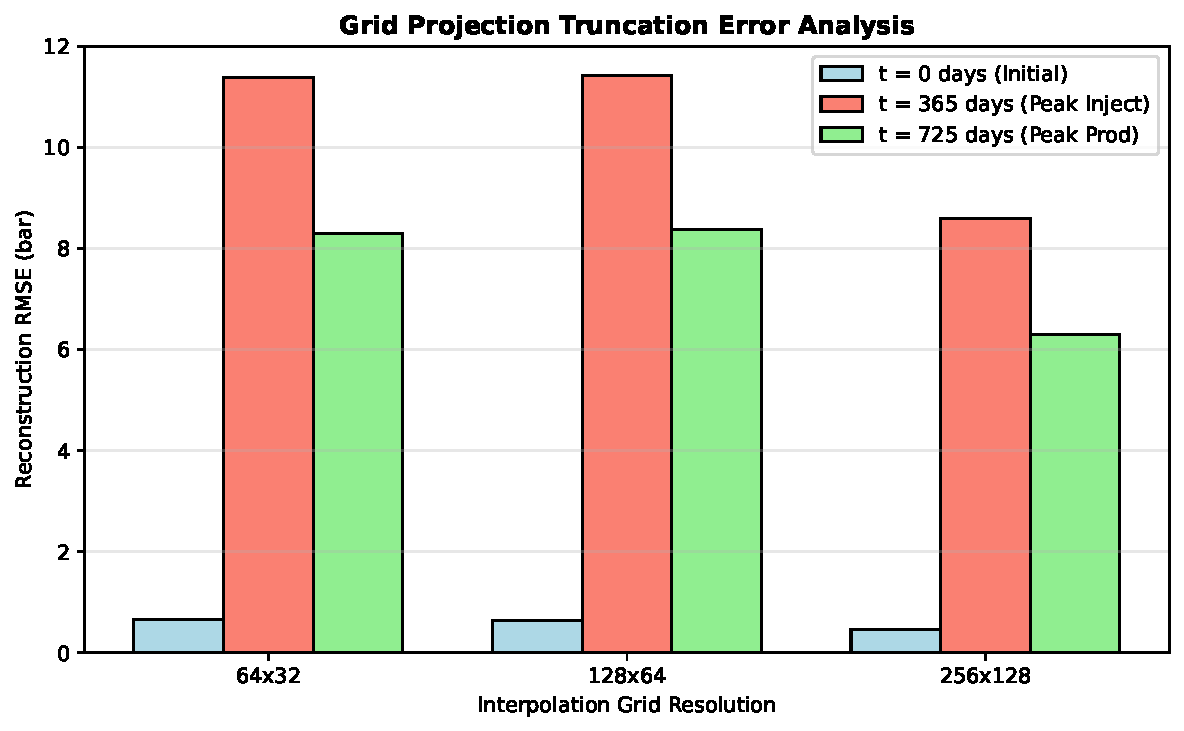
\includegraphics[width=0.95\columnwidth]{figures/fig6_interpolation_error}
    \caption{Pressure snapshot reconstruction RMSE (bar) comparing structured Cartesian grids ($64 \times 32$, $128 \times 64$, and $256 \times 128$) against the native 10,116-cell PEBI mesh, showing concentrated errors near wellbores.}
    \label{fig:interpolation_error}
\end{figure}
